\chapter{DELF}\label{delf_chapter}
Das Delf-Verfahren \cite{delf} von Noh, \mbox{Araujo} et al. bildet die Basis für die Experimente, die in dieser Arbeit durchgeführt werden. Im folgenden Abschnitt wird das Verfahren schrittweise im Detail erklärt. Beschrieben wird hierbei die Neuimplementierung in ihrer Basiskonfiguration, wie sie für den Experimentalteil dieser Arbeit verwendet wird. Unterschiede zu der von den Autoren zu Verfügung gestellten Implementierung\footnote[1]{\url{https://github.com/tensorflow/models/tree/master/research/delf}, zuletzt besucht 16.06.20}, sowie zu der Beschreibung des Verfahrens im Originalpapier \cite{delf} werden im hinteren Teil des Abschnitts erläutert. 
\\\\
Das Delf-Verfahren lässt sich in vier Phasen einteilen. Zu Beginn steht das sogenannte Finetuning. Hierbei wird ein vortrainiertes Modell, in unserem Fall ein ResNet-50 Netzwerk, auf einem neuen Datensatz weiter trainiert. Die Domäne der Bilder dieses Datensatzes sollte dabei möglichst nahe der späteren Retrievalaufgabe sein, damit das Modell lernen kann aussagekräftige Deskriptoren für diese Art von Bilden zu berechnen. In der nächsten Phase wird auf dem Model aufbauend ein Attention-Netzwerk trainiert welches die Güte berechneter Deskriptoren bewerten kann. In der dritten Phase werden für die Bilder der Datenbank, in der gesucht werden soll Deskriptoren extrahiert. Mit Hilfe des Attention-Netzwerks wird eine Vorauswahl besonders geeigneter Deskriptoren getroffen. Anschließend durchlaufen die Deskriptoren weitere Vorverarbeitungsschritte, mit denen sie in eine kompaktere Form gebracht werden. In der finalen Phase kann Delf aktiv genutzt werden. Es können nun Bilder als Suchanfragen gestellt werden. Delf vergleicht eine Anfrage mit allen Bildern des Datensatzes anhand der vorverarbeiteten Deskriptoren. Potentielle Matches zwischen Deskriptoren werden in einem letzten Schritt geometrisch verifiziert. Das Ergebnis einer Anfrage ist eine Rangliste der ähnlichsten Bilder, sortierte nach der Anzahl verifizierte Deskriptoren-Matches mit dem Anfragebild.

\section{ResNet}

Das Delf-Verfahren nutzt zur Erstellung von Deskriptoren ein Residuales Netzwerk (kurz ResNet). Bei der im Jahre 2015 vorgestellten ResNet Architektur \cite{resnet} von He, Zhang et al. handelt es sich um eine der meist genutzten tiefen CNN-Architekturen der aktuellen Forschung. ResNets finden Anwendung in unterschiedlichen Machine Learning Aufgaben, wie Klassifikation, Objektdetektion oder Image Retrieval. \\

Zeiler und Fergus haben gezeigt \cite{extraction_point_meaning}, dass CNNs mit wachsender Netzwerktiefe in der Lage sind komplexere Merkmale zu detektieren. Es scheint daher intuitiv für immer komplexere Aufgaben auch immer tiefere Netzwerke zu konstruieren. Allerdings stellt sich heraus, dass ab einem gewissen Punkt keine Verbesserung mehr mit dem bloßen aneinanderreihen von immer mehr Schichten erzielt werden können. Werden zu viele Schichten hinzugefügt sinkt dabei sogar die Trainingsperformanz. Mit dem rasanten Anstieg der Anzahl an Netzwerkparameter wird es immer schwieriger das Netzwerk zu optimieren. Parameter konvergieren deutlich langsamer zu einem Optimum und es gibt mehr lokale Minima in denen ein Netzwerk im Optimierungsprozess stecken bleiben kann. ResNets wirken diesem Problem mit der Einführung sogenannter Skip-Verbindungen entgegen. Hierbei werden zusätzliche Direktverbindungen im Netzwerk geschaffen, bei denen einige Schichten übersprungen werden. Fließt eine Eingabe an den Beginn einer Skip-Verbindung, so wird auf dieser die Identität der Eingabe mitgeführt. Parallel durchläuft die Eingabe die übersprungenen Schichten. Am Ausgangspunkt der Verbindung wird schließlich das Ergebnis der übersprungenen Schichten mit der Identität aufsummiert (siehe Abb. \ref{resnet}a). Durch die Bereitstellung der Identität hat das Netzwerk eine bessere Grundlage zur Optimierung und einzelne schlecht optimierte Schichten weniger negative Auswirkung auf die Netzwerkausgaben. Die Autoren stellen fest, dass CNNs bei Verwendung von Skip-Verbindung schneller zu einem Optimum konvergieren und dabei bessere Minima gefunden werden. 
\\
ResNets können in unterschiedlichen Konfigurationen erstellt werden. Das für Delf verwendete ResNet-50 besteht aus 49 faltenden gefolgt von einer vollvernetzen Schicht. Skip-Verbindungen überspringen jeweils drei Schichten. Die faltenden Schichten können in vier Blöcke eingeteilt werden. In jedem dieser Blöcke wird die Größe der entstehenden Featuremaps halbiert und die Merkmalstiefe erhöht (Siehe Abb.\ref{resnet}b). In der Implementierung dieser Arbeit wird die von Torchvision zur Verfügung gestellte ResNet-50 Architektur genutzt\footnote[2]{\url{https://github.com/pytorch/vision/blob/c2e8a00885e68ae1200eb6440f540e181d9125de/torchvision/models/resnet.py}, zuletzt besucht 16.06.20}. 
\begin{figure}
\label{resnet}
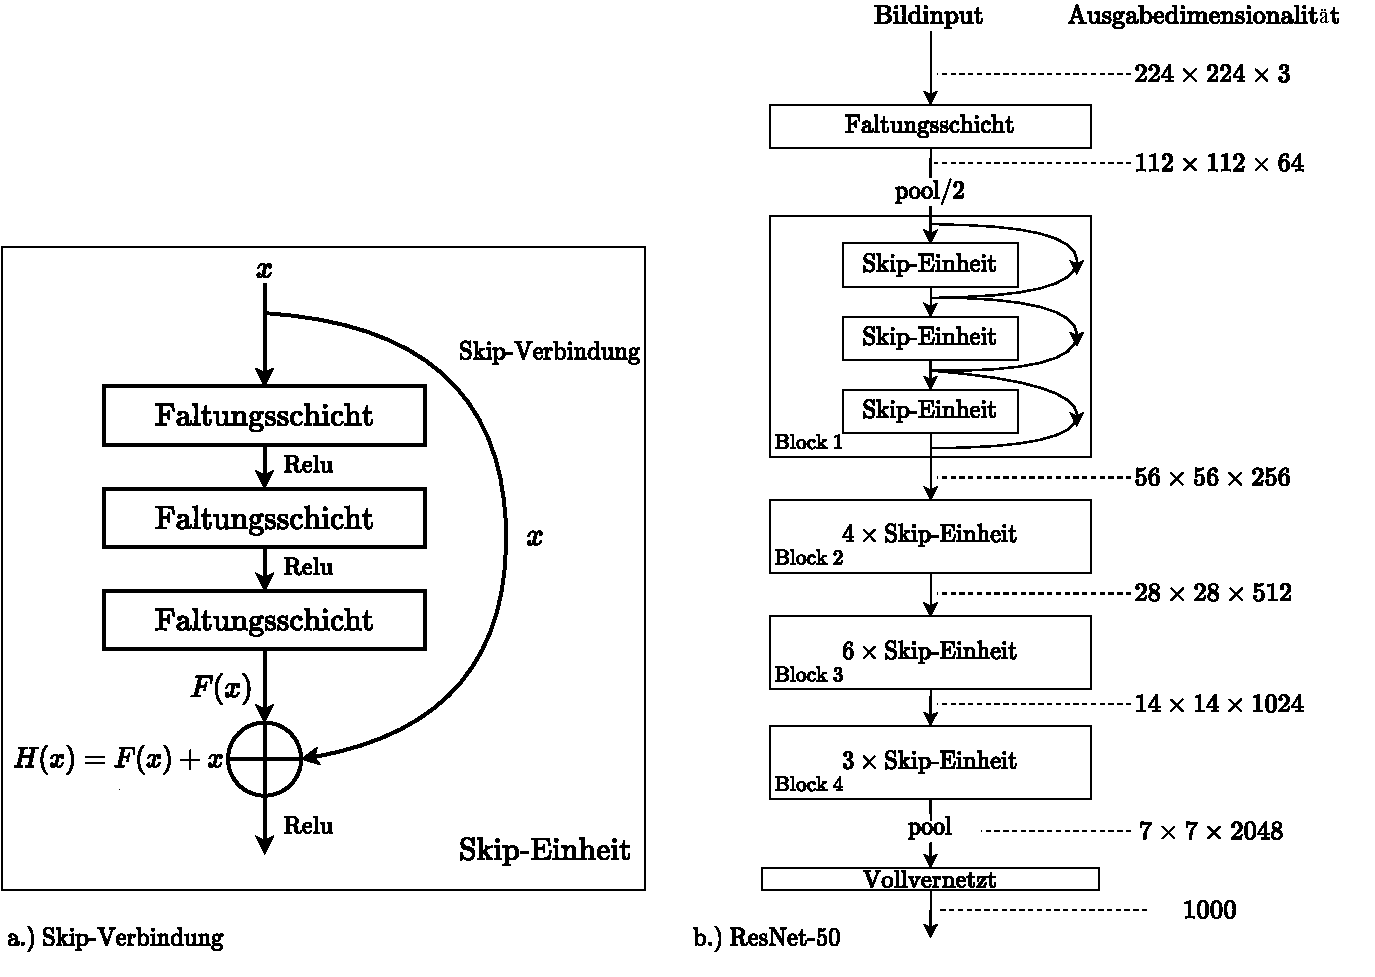
\includegraphics[scale=0.70]{resnet-50.pdf}
\caption{Aufbau der ResNet-Architektur (vgl. Fig.2, Fig.3 aus \cite{resnet})}
\end{figure}
